
\section{Betriebsszenarien}
\label{s:Betriebsszenarien}
Betriebsszenarien helfen die vorher beschriebenen Betriebs- und Infrastrukturkosten 
in Anwendung zu bringen und eine mögliche Entwicklung in naher Zukunft aufzuzeigen. 
Die Größe des Flughafens beeinflusst die Infrastrukturkosten. 
Bei einem größeren Flughafen werden die Betriebsdifferenzen deutlicher, 
da das \\Verkehrsaufkommen wesentlich höher ist.
Größere Flughäfen fertigen täglich mehr Flugzeuge als Regionalflughäfen ab, 
was dazu führt, dass mehr Abfertigungsplätze umgerüstet und versorgt werden müssen,
wodurch mehr Arbeitskräfte geschult werden müssen.

Deshalb wird der Flughafen Frankfurt für die Betriebsszenarien gewählt,
welcher als bedeutendes Luftverkehrsdrehkreuz fungiert
und zudem der größte Verkehrsflughafen Deutschlands ist.
Der Fraport meldete im Jahr 2023 insgesamt 423764 gewerbliche Flugbewegungen, 
was im Durchschnitt 1160 Flugbewegungen pro Tag ausmacht. 
Es wird angenommen, dass die Hälfte davon Abflüge sind, 
also müssen 580 Flugzeuge pro Tag abgefertigt werden.
%
Die Gesamtbewegungen teilen sich nach Entfernungen folgend auf \cite{fraport2023frankfurt}:
\begin{itemize}
    \item Kurzstrecken (bis 2500 km) sind bei 72,8 \%;
    \item Mittelstrecken (bis 6000 km) sind 9,3 \%;
    \item Langstrecken (ab 6000 km) die restlichen 17,9 \%. 
    \end{itemize}
Da nicht explizit definiert wird, welche Entfernungen die Flugzeuge zurücklegen, 
werden die Betriebskosten anhand vorher beschriebener Distanzen berechnet.
Dabei wird für Kurzstrecken eine Entfernung von 400 km 
und für Langstrecken eine Distanz von 6000 km angenommen.
Für Mittelstrecken werden die Werte der Langstreckenflüge verwendet, 
jedoch mit einer Distanz von 4000 Kilometern, 
sodass sich der Treibstoffverbrauch pro Stunde nicht ändert.

Anhand der zugrundeliegenden Informationen wird eine Flotte mit 580 Flugzeugen aufgestellt, 
in welcher alternative Antriebe eingesetzt werden.
Aufgrund der Flugeinschränkungen in der Nacht wird angenommen, 
dass die Flüge von 6 bis 24 Uhr gleichmäßig stattfinden. 
Wie bereits diskutiert wurde, können Kurzstrecken-Flüge durch 
den Einsatz von batteriebetriebenen Flugzeugen ersetzt werden, 
wobei hier als Ersatz auf SAF zurückgegriffen wird. 
Es ist nennenswert, dass nur ein Teil der tatsächlichen Nachfrage des Kurzstrecken-Bedarfs 
dadurch gedeckt werden kann. 
Die Mittel- und Langstrecken werden von Flugzeugen mit Wasserstoffturbine und SAF durchgeführt.
%
Durch die Betrachtung des tatsächlichen Flugplans sind die Spitzenstunden eines Tages zu ermitteln, 
bei welchen der Verkehrsfluss stärker ist, als im Durschschnitt.
In diesem Fall werden höhere Infrastruktur- und Betriebskosten erwarten zu sein.
Um die Interpretation zu erleichtern, wird in dieser Arbeit angenommen, 
dass stündlich die gleiche Anzahl an Flugzeugen am Flughafen abgewickelt werden. 
%
Die Aufteilung der Antriebe für jedes Szenario ist in der Abbildung \ref{betriebsszenarien} dargestellt.\\
%
\begin{figure}[h]
	\centering
	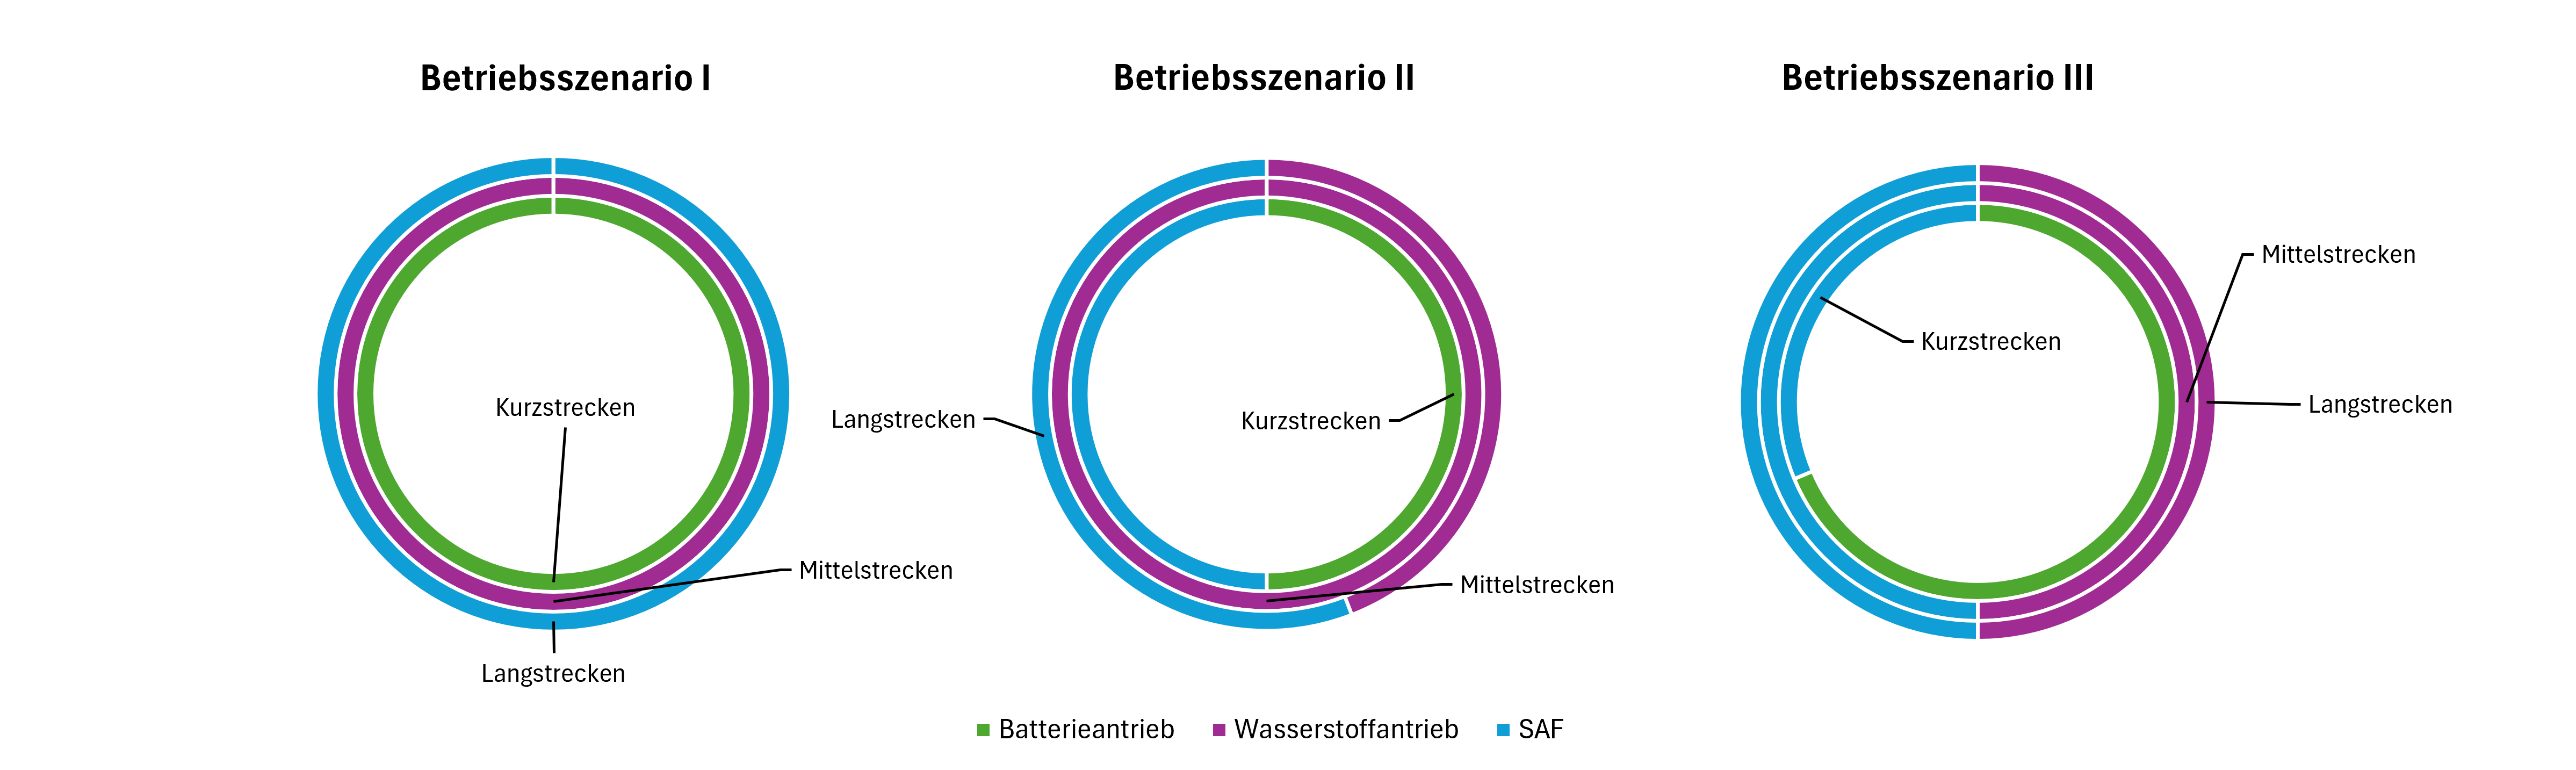
\includegraphics[width=1.0\linewidth]{Bilder/Betriebsszenarien.png}
	\caption[Betriebsszenarien]{Aufteilung der Flugzeugflotte nach Antriebsart}
	\label{betriebsszenarien}
\end{figure}
%
In dem \textbf{ersten Betriebsszenario} wird angenommen, dass:
\begin{itemize}
    \item Die Kurzstrecken werden vollkommen (72,8 \%) durch den Batterieantrieb, aufgrund Einschränkung des Reichweite
    \item Die Mittelstrecken werden vollkommen (9,3 \%) durch Wasserstoff und
    \item die Langstrecken werden vollkommen (17,9 \%) durch SAF betrieben.
\end{itemize}
Das \textbf{zweite Betriebsszenario} wird mit folgender Aufteilung berechnet:
\begin{itemize}
    \item 50 \% (36,4 \% absolut) der Kurzstrecken werden durch BA und 50 \% (36,4 \% absolut) durch SAF; 
    \item 100 \% (9,3 \% absolut) der Mittelstrecken werden, genau wie im ersten Szenario, komplett durch Wasserstoffflugzeuge und
    \item 10 \% der Langstrecken werden durch SAF und 7,9 \% durch Wasserstoff betrieben.
\end{itemize}
Das \textbf{dritte Szenario}:
\begin{itemize}
    \item 50 \% der Kurzstrecken werden durch BA und 22,8 \% mit SAF; 
    \item 50 \% (4,65 \% absolut) der Mittelstrecken werden mit WA und 50 \% (4,65 \% absolut) mit SAF und 
    \item 50 \% (8,95 \% absolut) der Langstrecken werden mit WA und 50 \% (8,95 \% absolut) mit SAF betrieben. 
\end{itemize} % für den rest der absoluten berechnungen bin ich zu dumm
%
Daraus ergibt sich die folgende Flottenaufteilung für die einzelnen Szenarien:
\begin{table}[h]
	\begin{center}
    \caption{Flugzeugzahlen in den Szenarien nach Antriebsart}
	\label{Szenarien_Fluege}
	\begin{tabular}{|c|c|c|>{\centering\arraybackslash}p{3cm}|c|}
		\hline
		\multicolumn{4}{|c|}{\textbf{Szenario I}} \\ \hline
		 & \textbf{Batterieantrieb} & \textbf{Wasserstoffantrieb} & \textbf{SAF} \\ \hline
		Kurzstrecke & 422 & - &-\\ \hline
      	Mittelstrecke & -  & 54 &- \\ \hline
		Langstrecke & - & - &104 \\ \hline
		\multicolumn{4}{|c|}{\textbf{Szenario II}} \\ \hline
		Kurzstrecke & 211 &- &211\\ \hline
      	Mittelstrecke &  - & 54 &- \\ \hline
		Langstrecke &- & 46  &58 \\ \hline
		\multicolumn{4}{|c|}{\textbf{Szenario III}} \\ \hline
		Kurzstrecke & 290 &- &132\\ \hline
      	Mittelstrecke &  - & 27 & 27 \\ \hline
		Langstrecke &  -& 52 &52 \\ \hline
	\end{tabular}
    \end{center}
\end{table}
